\documentclass[11pt]{report} % Use report class for chapters
\usepackage[a4paper, top=2cm, bottom=2cm, left=2cm, right=2cm]{geometry}
\usepackage{amsmath, amssymb} % For math formatting
\usepackage{titlesec} % For customising section titles
%\titlespacing{\chapter}{0pt}{-30pt}{20pt} % Adjust top spacing
\usepackage{fancyhdr} % For headers and footers
\usepackage{hyperref} % For a clickable table of contents and references
\usepackage{tocloft} % For customising the table of contents
\usepackage{setspace} % For line spacing
\usepackage{booktabs}
\renewcommand{\abstractname}{Declaration} % Change "Abstract" to "Summary"

% Formatting title sections
\titleformat{\chapter}[hang]{\bfseries\LARGE}{Chapter \thechapter}{1em}{}
\titleformat{\section}[hang]{\large\bfseries}{\thesection}{1em}{}

% Customise TOC spacing
\renewcommand{\cftchapdotsep}{1.5} % Adjust dots in TOC

% Line spacing
\onehalfspacing % Set 1.5 line spacing

% Header and footer
\pagestyle{fancy}
\fancyhf{}
\fancyhead[L]{\slshape \leftmark} % Chapter title on left
\fancyfoot[C]{\thepage} % Page number at center

% Math and Symbols
\usepackage{amsmath, amssymb} % For math environments and symbols

% Graphics and Floats
\usepackage{graphicx} % Include images
\usepackage{float} % Improved float handling

% Hyperlinks
\usepackage{hyperref} % For clickable hyperlinks

% Code Listings
\usepackage{listings}
\usepackage{xcolor}

\lstset{
    language=R,                     % Set language to R
    basicstyle=\ttfamily\Huge,      % Increase font size (change to Huge, Large, normalsize)
    breaklines=true,                 % Enable automatic line breaking
    breakatwhitespace=true,          % Allow line breaks at spaces
    keepspaces=true,                 % Keep spaces in text
    columns=fullflexible,            % Fix alignment
    frame=single,                    % Adds a frame around the code
    backgroundcolor=\color{gray!10},  % Light gray background for readability
    keywordstyle=\color{blue},        % Blue for function names
    commentstyle=\color{green!50!black}, % Green for comments
    stringstyle=\color{red},          % Red for strings
}

% Citations
\usepackage[numbers, super]{natbib} % For citation styles
% Remove \usepackage{cite}, as natbib replaces it.

% Images
\usepackage{subcaption}
%\captionsetup[subfigure]{font=scriptsize}
\captionsetup[figure]{font=small}

\usepackage{xfp} % For calculations in LaTeX
\usepackage{xcolor} % For color coding

% Define colours
\definecolor{darkgreen}{rgb}{0.0, 0.5, 0.0}
\definecolor{lightgreen}{rgb}{0.0, 0.75, 0.0}
\definecolor{yellow}{rgb}{1.0, 0.84, 0.0}
\definecolor{red}{rgb}{1.0, 0.0, 0.0}

\newcommand{\classifyFit}[1]{%
  \ifnum\fpeval{#1 <= 0.5}=1 \textcolor{darkgreen}{Excellent}% 
  \else\ifnum\fpeval{#1 <= 0.6}=1 \textcolor{lightgreen}{Good}% 
  \else\ifnum\fpeval{#1 <= 0.7}=1 \textcolor{yellow}{Satisfactory}% 
  \else \textcolor{red}{Unsatisfactory}% 
  \fi\fi\fi
}

\lstset{
    language=R,
    basicstyle=\ttfamily\scriptsize, % Use smaller font size
    flexiblecolumns=true,            % Allows font to shrink for long lines
    showstringspaces=false,          % Do not show spaces in strings
    frame=none,                      % No frame around code
    numbers=none,                    % No line numbers
    breaklines=false,                % Force code in one line
    literate={~}{{\texttildelow}}1
}

% Begin document
\begin{document}


\begin{titlepage}
    \begin{center} 
        \hfill \break
         \vspace{5mm}
         
        
\includegraphics[width=0.6\textwidth]{Durham_Uni_Name.png}   
       
        \vspace{1cm}
        \LARGE
            Department of Mathematical Sciences \\
            Deep Learning and Artificial Intelligence - (MATH4267)
        
        \linethickness{0.5mm}
        \Huge
            \line(1,0){250}\\
            \textbf{Summative Assignment}\\
            \line(1,0){250}
        
    \end{center}  

    \begin{minipage}[t]{0.47\textwidth}\centering
        {\Large \textbf{Author}:\\
        Raul Unnithan}\\
    \end{minipage}
    \hfill
    \begin{minipage}[t]{0.47\textwidth}\centering
        {\Large \textbf{Supervisor}:\\
        Doctor James Liley}
    \end{minipage}

    \vfill  % Pushes date to the bottom

    \begin{center}
        \large \today  
    \end{center}
    
\end{titlepage}


\begin{abstract}
This piece of work is a result of my own work and I have complied with the Department’s guidance on multiple submission and on the use of AI tools. Material from the work of others not involved in the project has been acknowledged, quotations and paraphrases suitably indicated, and all uses of AI tools have been declared.
\end{abstract}


\tableofcontents
\newpage

% Chapters
\chapter{Part 1 %- about 4 pages
}

The first part of this assignment looks at Paper 3: On the Convergence Rate of Gaussianization with Random Rotations by Draxler et al. (2023).

\section{Background}
The paper focuses on generative modelling. This modelling approach aims to learn an underlying data distribution in order to generate new, realistic samples. Popular approaches include generative adversarial networks (GANs), variational autoencoders (VAEs), normalising flows, and diffusion models. This paper focuses on Gaussianization, which is a specific type of normalising flow, and how it converges with random rotations.

Gaussianization maps data to a standard normal distribution using a sequence of invertible transformations—specifically, alternating random orthogonal rotations with component-wise non-linear functions. Unlike most deep generative models, it does not require backpropagation, making it more efficient.
However, this approach comes with a fundamental limitation, which is that as the dimensionality of the data increases, convergence becomes significantly slower when using random rotations. In this paper, the authors find that the number of layers required increases with dimensionality.

This paper is the first work to derive an explicit convergence rate for Gaussianization. One of its key contributions is that it establishes that the number of layers required for effective Gaussianization increases at least linearly with data dimension when using random rotations. It also considers rotations learned from data but discovers that simpler methods overfit or focus on spurious (fake) non-Gaussian directions, especially in high dimensions. Finally, the paper highlights that Gaussianization does not track dependencies among features in high dimensions, thus making it ineffective.

One direction for future work following this paper is to come up with better rotation strategies that enable convergence in high-dimensional spaces. This would involve learning rotations that encode patterns in the data without overfitting to noise or irrelevant features. Another direction could be looking into how to combine Gaussianization with models that are able to focus more on interactions between features, such as coupling layers.

%Finally, it empirically determines the scaling behaviour on real-world datasets, observing a similar linear increase in complexity with dimension and favourable scaling for certain distributions.

\section{New Real-World Application}
A potential new real-world application of the Gaussianization with Random Rotations is generating high-quality synthetic tabular data for healthcare applications.\cite{pezoulas2024synthetic} This includes patient datasets with lots of continuous and numerical predictors (such as lab measurements and vitals), where preserving the statistical properties of the original dataset while ensuring privacy is critical. Gaussianization is well-suited for such tasks because it uses layer-wise transformations with rotations and 1D non-linear functions, which can be trained efficiently without backpropagation and perform well even with limited training data.

\noindent The primary objective in this application is to minimise the Kullback-Leibler (KL) divergence between the latent code \( q(z) \) and the standard multivariate normal distribution \( \mathcal{N}(\mathbf{0}, \mathbf{I}) \):
\begin{equation}
D_{\mathrm{KL}}(q(z) \, \| \, \mathcal{N}(\mathbf{0}, \mathbf{I})) = \int q(z) \log \frac{q(z)}{\mathcal{N}(z;\mathbf{0}, \mathbf{I})} \, dz.
\label{KL}
\end{equation}

\noindent Equation \ref{KL} is the Gaussianization loss function from Section 3.1 of the paper. This equation measures how far the transformed data is from an ideal Gaussian distribution. Reducing the KL divergence implies a better match to the distribution, leading to high-quality sample generation and reliable density estimation.

Reducing the KL divergence in this context is beneficial for several reasons. First, synthetic data can replicate the underlying behaviours of the patient data without copying real individuals, thus aligning with privacy regulations such as the General Data Protection Regulation. Second, for rare diseases or under-represented groups, the model can generate realistic but new samples to build on the dataset. Finally, Gaussianization's use of dimension-wise transforms and random rotations enables easier checks compared to black-box models like GANs.
%Finally, in low-data regimes, Gaussianization is preferable to neural-network-based generative models, as it does not require lots of parameters or gradient-based training.

Gaussianization with Random Rotations applies to these datasets in the following way. Given a real tabular dataset \( x \sim p(x) \), we learn an {invertible transformation} \( f_\theta(x) \) such that:
  \[
  z = f_\theta(x) \sim \mathcal{N}({0}, \mathbf{I}).
  \]
This means the data is mapped to a {latent Gaussian space} via a composition of randomised {rotations}, \( f_{\mathrm{rot}} \), and {non-linear 1D transformations}, \( f_{\mathrm{dim}} \), as shown in this equation:
\[
  f_{\mathrm{block}}(x) = (f_{\mathrm{dim}} \circ f_{\mathrm{rot}})(x).
\]
The Gaussianization structure then removes dependencies by separating them into global dependence, \( \mathcal{D} \), and {marginal losses}, \( \mathcal{J}_i \), for each dimension: 
\begin{align*}
\mathcal{L} &= \mathcal{D}_{\text{KL}}\left( q(z) \middle\| \mathcal{N}(0, \mathbf{I}) \right) \\
            &= \underbrace{\mathcal{D}_{\text{KL}}\left( q(z) \middle\| q(z_1) \cdots q(z_D) \right)}_{\text{Dependence } \mathcal{D}} 
            + \underbrace{\sum_i \mathcal{D}_{\text{KL}}\left( q(z_i) \middle\| \mathcal{N}(0, 1) \right)}_{\text{marginal loss } \mathcal{J}_i}.
\end{align*}
\noindent The rotations \( Q \in O(D) \) are used to {redistribute dependence} so that as much redundancy as possible is captured by the 1D transformations: \(f_{\text{rot},\, Q}(x) = Qx.
\)

%In practice, the choice of rotation matrix, $Q$, plays an important role in the balance between marginal and dependence terms of the KL divergence. In principle, if we knew the best rotation $Q*$ that would completely diagonalise the structure, then this transformation could be matched to the target Gaussian distribution in one layer. But for practical datasets, such as those involving healthcare records, this best rotation is either unknown or impossible to calculate. Hence, we most commonly use random rotations to expose non-Gaussian structure. The rotation then serves to redistribute latent dependences in a way that makes 1D non-linear mappings most effective at each level.

Next, the Gaussianization model needs to be trained. This is done using iterative or end-to-end training. 
Iterative training involves adding layers one by one. The dataset is used to train the first block, $f_\text{block}$, to maximally reduce
the loss in Equation \ref{KL}. The second block is then trained with the data transformed by the first layer.
In end-to-end training, concatenate a pre-specified number of blocks at initialisation.\cite{meng2020gaussianization} The parameters of each block are then trained jointly using Equation \ref{KL}.
%The advantage of end-to-end training is that blocks can collaborate, as the training signal is the gradient of the entire pipeline and not just of a single block.

Iterative training has the advantage that there are fast approaches for learning the 1D transforms. In practice, end-to-end training requires fewer layers than
iterative training when learning a given distribution in low dimensions.\cite{meng2020gaussianization} As the dimension increases, however, the convergence of the training levels off. Therefore, this paper uses iterative training.
% State-of-the-art Gaussianization results in high dimensions (MNIST, CIFAR10) are currently held by iterative training with SINF (Dai \& Seljak, 2021).

Once the model is trained, sample \( z' \sim \mathcal{N}(0, \mathbf{I}) \) and use the inverse transformation \( x' = f_\theta^{-1}(z') \).
This returns {synthetic tabular data} \( x' \) that retains the structure of the original dataset.

\section{Theorem 1}
%\subsection*{Paper iii – Theorem 1}
Consider a tabular healthcare dataset where each sample is represented by a high-dimensional feature vector \( \mathbf{x} \in \mathbb{R}^D \), representing a patient with \( D\) pieces of medical information (such as blood pressure, heart rate, cholesterol, etc). %We assume that the underlying data distribution is approximately multivariate Gaussian, \( p(\mathbf{x}) = \mathcal{N}(\mathbf{0}, \mathbf{\Sigma}) \), where \( \mathbf{\Sigma} \) is an unknown but full-rank feature covariance matrix. This distribution also has the following further assumptions: the covariance is normalised, so \( \operatorname{tr} \mathbf{\Sigma} = D \), and the eigenvalues of the covariance matrix \( \mathbf{\Sigma} \) are distinct: \( \lambda_i \neq \lambda_j \) for \( i \neq j \).

%A practitioner wishes to use Gaussianization with random rotations to map this data into a latent Gaussian space for density estimation and synthetic data generation.

The assumptions of Theorem 1 are that the data is drawn from a centred multivariate Gaussian distribution, \( p(\mathbf{x}) = \mathcal{N}(\mathbf{0}, \mathbf{\Sigma}) \), with a full-rank covariance matrix \( \mathbf{\Sigma} \in \mathbb{R}^{D \times D} \). Therefore, the parent population of patient information follows this structure in the example set out above.
This distribution must also follow 2 further assumptions. Assumption 1 requires that the covariance is normalised, i.e., \( \operatorname{tr} (\mathbf{\Sigma}) = D \), while Assumption 2 ensures that all eigenvalues of \( \mathbf{\Sigma} \) are distinct (\( \lambda_i \neq \lambda_j \) for \( i \neq j \)). 

The aim of Theorem 1 is to exactly represent this distribution using a sequence of Gaussianization layers, where each Gaussianization block consists of a random orthogonal rotation followed by independent 1D non-linear transforms. The transformations are linearised and parameter-counted (ignoring non-linearities for the lower bound).

Theorem 1 establishes that, under the above assumptions, Gaussianization, with $Q$ random rotations, must use at least $L$ Gaussianization layers to exactly represent the target Gaussian distribution, \( p(\mathbf{x})=\mathcal{N}(\mathbf{0}, \mathbf{\Sigma}) \), almost surely, where:
\[
L \geq \frac{1}{2}(D + 1).
\]
This result is surprising because it reveals an inherent inefficiency in random-rotation Gaussianization: the required number of layers scales linearly with dimension, even for Gaussian inputs, which already have the ideal target of Gaussianization. %Previous universal approximation theorems guaranteed convergence weakly but did not quantify how many layers are required.\cite{ismailov2024universal} Theorem 1 fills that gap.

Theorem 1 gives, for the first time, a strict lower bound on the KL divergence, assuming a given number of layers for random rotations $Q\in O(D)$. It says that Gaussianization may require an extremely large number of layers to approximate even simple distributions like a full-covariance Gaussian matrix. In practice, this means those using Gaussian with randomised rotations should either use more expressive transformation layers, such as coupling or attention-based layers, along with this Gaussianization approach. %or consider hybrid approaches that better capture inter-dimensional dependencies with fewer layers.
This insight is especially relevant when working with high-dimensional data, where computational efficiency and layer count directly affect training time and sample quality.

\begin{figure}[H]
    \centering
    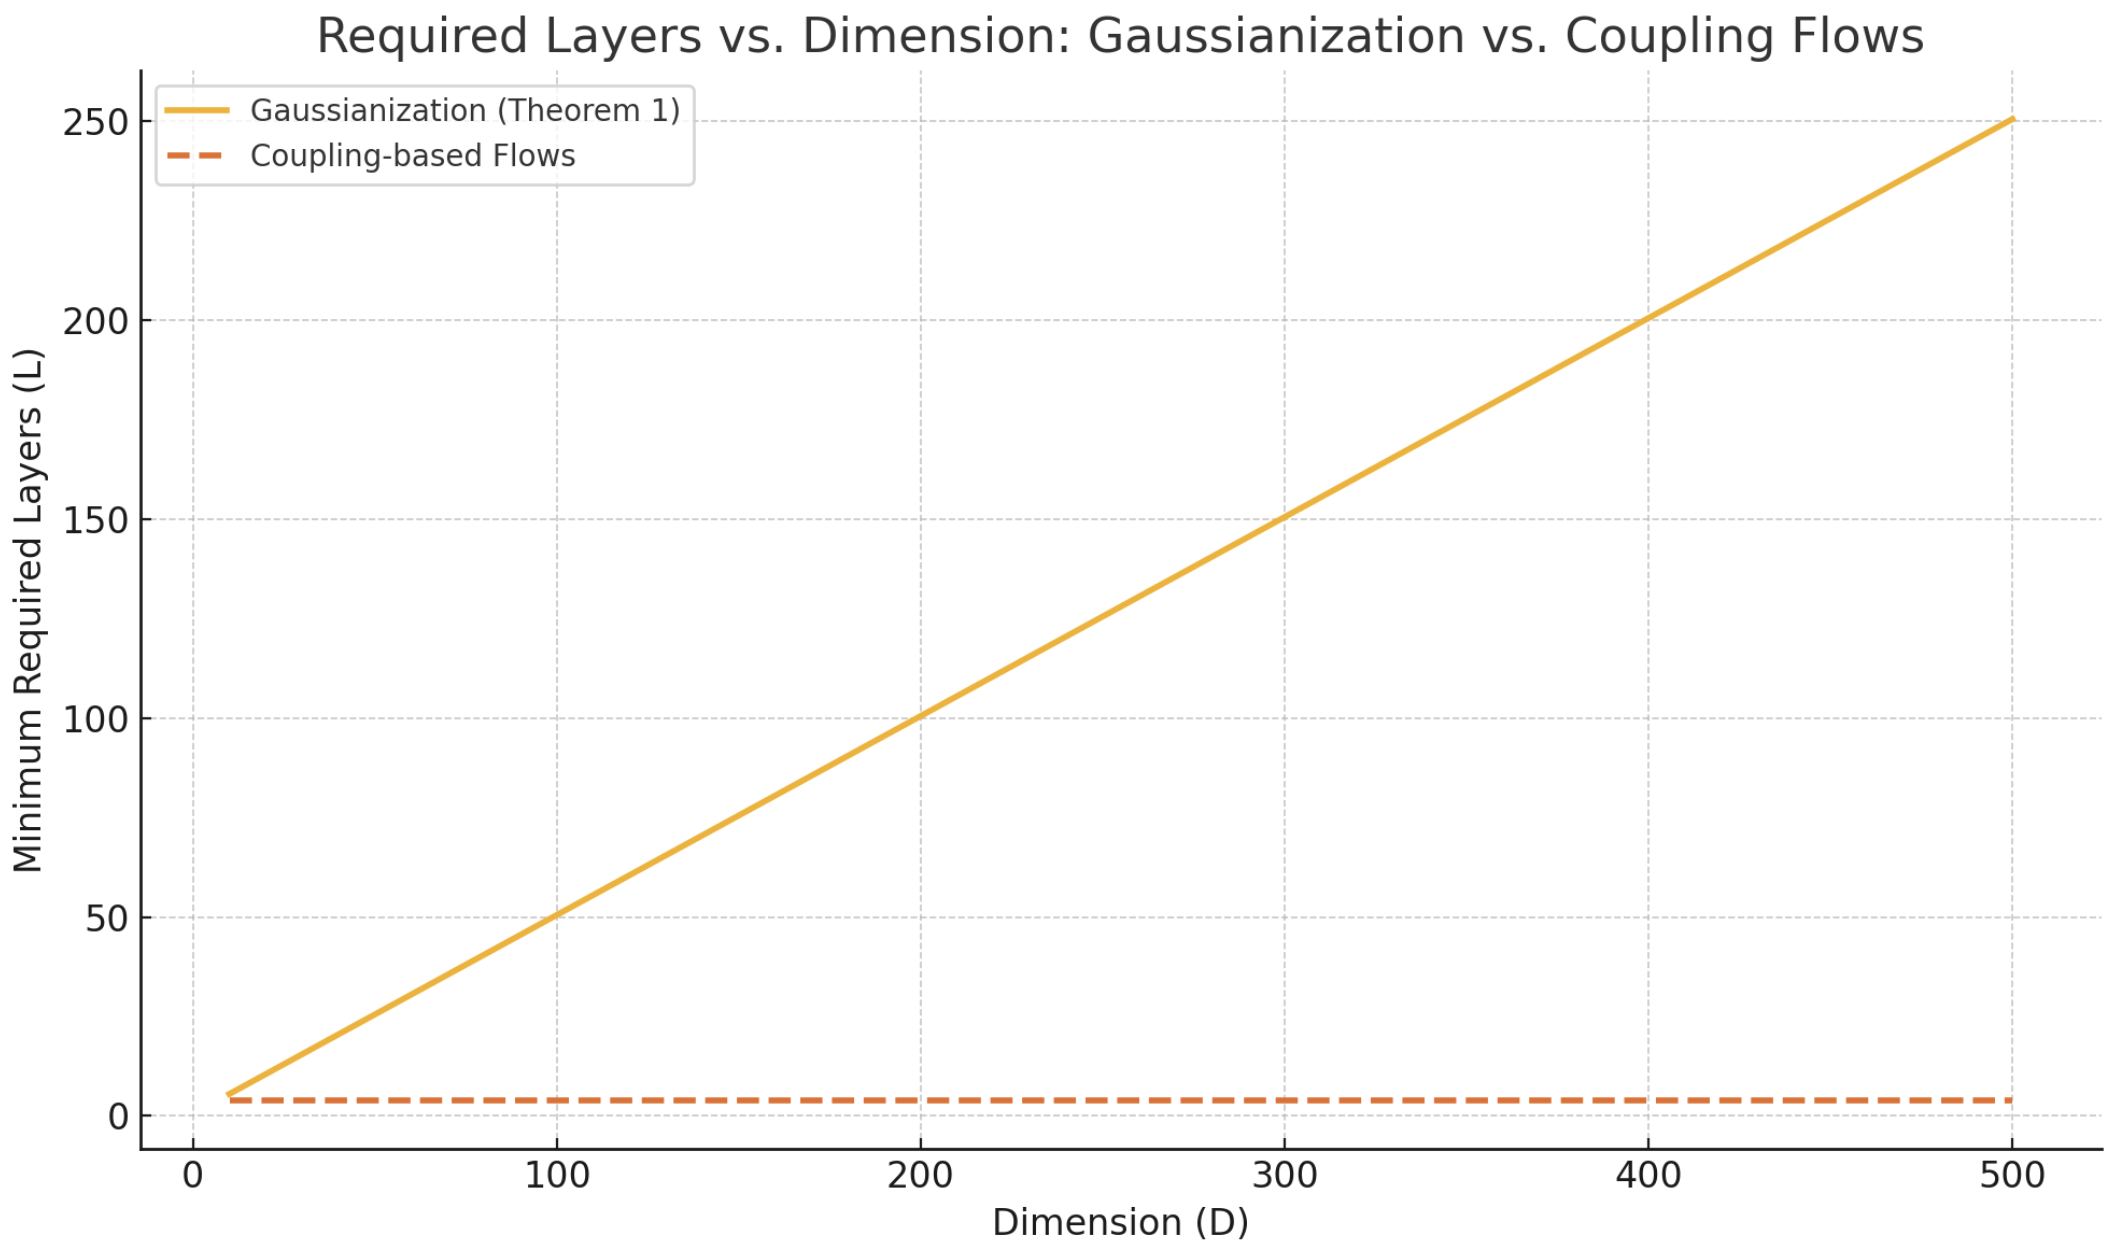
\includegraphics[width=0.55\linewidth]{Gaussianization vs. Coupling Flows.png}
    \caption{Gaussianization vs. Coupling Flows}
    \label{fig:Gaussianization vs. Coupling Flows}
\end{figure}
\noindent Figure \ref{fig:Gaussianization vs. Coupling Flows} illustrates the insight from Theorem 1. 
The solid line shows how the number of required Gaussianization layers grows linearly with dimension, as predicted by the theorem. In contrast, the dashed line represents coupling-based flows, which need only a constant number of layers. 

\noindent Theorem 1, therefore, shows the theoretical and practical issues of the hidden costs of scaling Gaussianization in high-dimensional data domains such as in medicine.

\section{Why are Equation 20, Theorem 2 and Figure 4 of interest?}

Equation (20) states that the number of coupling layers \( L_{\mathrm{cpl}} \) required to Gaussianise multivariate Gaussian data using coupling-based flows is constant with respect to the data's dimensionality:
\[
L_{\mathrm{cpl}} = \Theta(1).
\tag{20}
\]
This implies that the convergence rate of coupling blocks does not worsen as the dimension increases. Also, this means that on Gaussian data, Gaussianization requires more layers than coupling blocks because the
layers do not model dimension interdependencies (see Figure~\ref{fig:Gaussianization vs. Coupling Flows} for a comparison of this).

This result directly contrasts with Gaussianization using random rotations, where the number of layers needed grows linearly with dimension (\( \Omega(D) \)). This part of the paper compares how quickly different transformation approaches, such as Gaussianization and coupling flows, converge and Equation (20) is a benchmark for this comparison.

This is useful to someone using Gaussianization with randomised rotations when working in high dimensions, because while Gaussianization may be conceptually simple and interpretable, it is not efficient at scale. Equation (20) highlights that coupling-based methods are more suitable when working with high-dimensional Gaussian-like data due to their dimension-independent convergence.

%\vspace{1em}

Theorem 2 establishes a convergence rate bound for Gaussianization with random rotations under Assumption 1. 
Note: Assumption 1 requires that the covariance is normalised, i.e., \( \operatorname{tr} (\mathbf{\Sigma}) = D \).

Theorem 2 states that given a multivariate Gaussian distribution
$p(x) = N (0, \mathbf{\Sigma})$ under Assumption 1. Then, in the case $\mathcal{L} << 1$, the expected loss after $L$ iterative Gaussianization blocks with random rotations is approximately:
\[
\mathbb{E}_{Q_{1\dots L}\in O(D)}[\mathcal{L}^{(L)}] \leq \left(1 - \frac{2}{D + 2} \right)^L \mathcal{L}.
\]
From this, it follows that the number of layers required to reduce the loss by a fixed ratio scales at least linearly with the data dimension, $L = \Omega(D)$:
\[
L \geq \frac{\log(\mathcal{L}' / \mathcal{L})}{\log\left(1 - \frac{2}{D + 2}\right)} 
\approx \log(\mathcal{L} / \mathcal{L}')\frac{D + 1}{2} = \Omega(D).
\]
This result formalises a key limitation of Gaussianization in the iterative setting. Even for ideal Gaussian inputs, the model cannot converge efficiently using a fixed number of layers. This further supports Theorem 1's conclusion and reinforces the paper's central idea, which is the inefficiency of Gaussianization in high-dimensional spaces.

For those applying Gaussianization with randomised rotations, Theorem 2 quantifies its scalability issue. While the method is simple and does not require backpropagation, achieving low KL divergence may require a large number of layers as $D$ increases, which extends factors such as training time.
%\vspace{1em}
\begin{figure}[H]
    \centering
    \renewcommand{\thefigure}{4} % <-- Force label to be Figure 4
    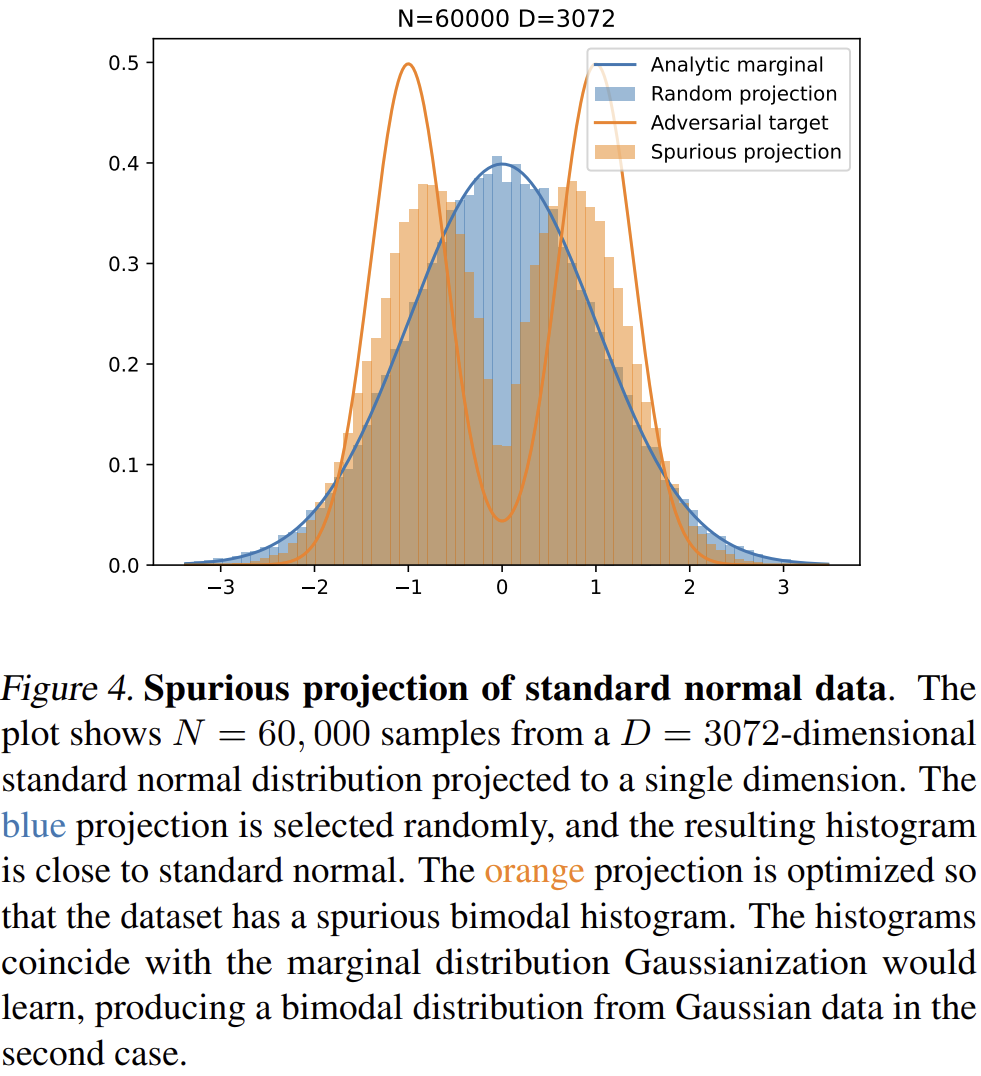
\includegraphics[width=0.4\linewidth]{Figure 4.png}
    \caption{Spurious projection of standard normal data.}
    \label{fig:spurious-projection}
    \addtocounter{figure}{-1} % <-- Prevents LaTeX from advancing to Figure 5
\end{figure}
\noindent
Figure~\ref{fig:spurious-projection} shows that even when data is sampled from a high-dimensional standard normal distribution, some one-dimensional projections can yield spurious histograms. The above figure shows a spurious bimodal histogram - specifically, the projection is of the form:
\[ x_{\text{proj}} = w^\top x, \quad \|w\| = 1, x \sim \mathcal{N}(0, \mathbf{I})\] 
with N fixed samples from a D-dimensional standard normal.
We construct $w$ such that the projection of the fixed data (in blue) is as close as possible to the bimodal distribution (in orange).
Although no such \( w \) exists in the asymptotic limit \( N \to \infty \), the optimisation finds such a projection in finite datasets. 

This plot shows the risk of using only marginal Gaussianization, since if Gaussianization only relied on marginal statistics, it would learn this bimodal shape as if it mattered.
It also confirms the theoretical argument that marginal convergence is insufficient because significant interdependencies among various dimensions can be neglected. This supports the need to evaluate convergence using the full KL divergence rather than only marginal fits.

Ultimately, this figure warns those applying Gaussianization with randomised rotations against assessing generative models using only visual or one-dimensional summary statistics, especially in areas like synthetic healthcare data, where such approaches can lead to misleading conclusions about model quality.

\chapter{Part 2}
\section{Task A: Character Classification Using Transfer Learning}
My first approach was to establish a basic convolutional neural network (CNN) model that consisted of two convolutional layers with ReLU activations, max pooling, and a dense softmax output layer. This model achieved a validation accuracy of near 75\%, but it plateaued really early. I then attempted to improve performance by adjusting hyperparameters (including the number of filters, dropout rate, and fully connected layer size) but the model’s performance actually worsened, indicating overfitting. 

With these limitations, I proceeded to transfer learning using MobileNetV2, which is a pre-trained CNN that was trained with the ImageNet dataset. The model was then loaded with a frozen convolutional base to maintain its learned visual features. I then appended a custom classification head made up of a global
average pooling layer, a dropout layer (of rate 0.5), a dense layer with 128 ReLU functions, and a final
softmax output layer with 6 units, one for each character.

In order to be compatible with MobileNetV2, I preprocessed the input data by normalising pixel
intensities to the [0, 1] range, copying the grayscale channel to mimic RGB, and resizing each
resized the image to 96 × 96. The labels were integers (0–5) and subsequently one-hot encoded. The model
was trained for 20 epochs using the Adam optimiser with a batch size of 32, and an 80–20 stratified
train-validation split.

In order to reduce overfitting, I froze the pre-trained convolutional layers and added dropout (rate 0.5) in the custom classification head. These regularisation techniques helped to improve generalisation without
with a large quantity of trainable parameters.

Ultimately, the model attained a validation accuracy of approximately 90.91\%, significantly exceeding
the initial CNN. This corroborated that the transfer learning methodology proved to be more effective here.
I believe this was due to the strong feature representations MobileNetV2 had learned on large-scale
visual information, which generalised well even after fine-tuning on a small dataset.

\section{Task B: Conditional Variational Autoencoder}
I implemented a Conditional Variational Autoencoder (CVAE) to generate the 500 images for each character. I selected it over GAN-based models because of how it controls the latent space and its explicit regularisation via KL divergence. I iteratively refined the CVAE based on early results, where shallower models failed to distinguish certain characters (especially E and F) even after hundreds of training epochs.

The model used three convolutional layers in the encoder to downsample inputs to a 4×4 latent representation. I set the latent dimensionality to 50 to balance expressiveness and regularisation. In the decoder, I used transposed convolutions to upscale to 32×32, then manually cropped the result to 28×28 within the decoder to match the original input dimensions.

\noindent Label information was then injected at three points. First, it was appended as additional channels to the image tensor in the encoder. Then, the information was concatenated with the latent code in the encoder and finally it was merged into the visual output. This final label injection was critical because without it, several characters produced near-identical or entirely blank outputs. Injecting label information directly into the spatial layers helped guide the decoder to focus on the intended character, rather than leaving character differences to emerge from the latent space alone.

The forward pass combined encoding, reparameterisation and decoding into a fully differentiable pipeline. I trained the model for 1000 epochs using the Adam optimiser with a learning rate of $10^{-3}$. This was applied with a custom loss which summed binary cross-entropy and KL divergence the and analytic KL term.
When training, I printed loss values every
100 mini-batches and looked at sample generations for each character (A-F) at regular intervals to track progress. Quality
plateaued after 1000 epochs, suggesting that further training provided diminishing returns.

I mitigated overfitting primarily via regularising the CVAE, in particular through the KL divergence term. This constrained the latent space to remain near a standard Gaussian, preventing the model from merely memorising the training data. I also maintained a moderate depth and filter sizes of the decoder to prevent over-parameterising, and refrained from using dropout or data augmentation so that clear character features would be preserved. Despite the model's smaller size relative to contemporary generative networks, randomness that arose as a consequence of sampling in the latent space performed as an implicit mechanism of regularisation.

I briefly considered a Conditional GAN, which could produce sharper images, but decided against it due to the small dataset and high risk of mode collapse. GANs usually need careful tuning to keep the generator and discriminator balanced, and getting them to follow character labels properly can be unreliable without extra components. In contrast, the CVAE was a lot more flexible as the generation process at every stage could be guided using the labels, and it also allowed me to explore how changes in the latent space affected the output. Ultimately, the model was easy to train and consistently produced diverse but character-specific results without much fine-tuning.

Looking back, adding a simple adversarial component to sharpen the images could have helped without losing character control. But for this task, the CVAE gave a good balance between producing accurate character outputs and keeping the model easy to train and understand.

% Bibliography
\makeatletter
\renewcommand\@biblabel[1]{#1.} % Change numbering style to 1.
\makeatother
\bibliographystyle{unsrt}
\bibliography{references}

\end{document}
